\documentclass[12pt]{article}
\usepackage[utf8]{inputenc}
\usepackage{geometry}
\geometry{a4paper, margin=1in}
\usepackage{tikz}
\usetikzlibrary{shapes.geometric, arrows.meta, positioning}
\usepackage{microtype}
\usepackage{booktabs}
\usepackage{amsmath}
\usepackage{amssymb}

% Custom formatting
\usepackage{titlesec}
\titleformat{\section}{\large\bfseries\sffamily}{\thesection}{1em}{}
\renewcommand{\familydefault}{\sfdefault}

\begin{document}

% --- Page 1: Highlights ---
\thispagestyle{empty}
\begin{center}
    \vspace*{1cm}
    {\large\bfseries\sffamily\color{blue!80} RESEARCH HIGHLIGHTS} \\[1.5em]
    {\large\bfseries Autonomy at the Edge: Governance, Risk, and International Policy Frameworks for\\ AI-Driven Deep Space Communications} \\[1.0em]
    {\small Jason Pandian$^{1}$ and I. Kala$^{2}$} \\[0.5em]
    {\scriptsize $^{1}$Department of Information Technology, Nehru Institute of Technology, India \\
    $^{2}$Department of Computer Science and Engineering, PSG Institute of Technology and Applied Research, India} \\
    \rule{\linewidth}{1.5pt}
    \vspace{2cm}
\end{center}

\begin{itemize}
    \setlength{\itemsep}{1.5em}
    \item \textbf{Spectrum Policy Gaps:} Analyzes acute policy gaps in ITU regulations regarding dynamic, space-grade AI spectrum allocation and the Outer Space Treaty's access principles.
    \item \textbf{Physical Infrastructure Asymmetries:} Exposes geopolitical asymmetries in deep space ground network infrastructure and proprietary software control (NASA, ESA, CNSA, ISRO, and JAXA complexes).
    \item \textbf{Algorithmic Bias Modeling:} Models a multinational Martian dust storm scenario to demonstrate systemic bias in autonomous ``data triage'' loops.
    \item \textbf{Explainable AI (XAI) Framework:} Proposes an auditable, cryptographic Explainable AI (XAI) framework for spacecraft downlink priority and write-once decision logs.
    \item \textbf{COPUOS Code of Practice:} Drafts a concrete ``International Code of Practice for Autonomy in Deep Space Telecommunications'' under UN COPUOS to establish algorithmic transparency and dynamic envelopes.
\end{itemize}

\newpage

% --- Page 2: Graphical Abstract ---
\thispagestyle{empty}
\begin{center}
    \vspace*{0.5cm}
    {\large\bfseries\sffamily\color{blue!80} GRAPHICAL ABSTRACT} \\[1.0em]
    {\large\bfseries Autonomy at the Edge: Governance, Risk, and International Policy Frameworks for\\ AI-Driven Deep Space Communications} \\[1.5em]
    \rule{\linewidth}{1.5pt}
    \vspace{2.5cm}
\end{center}

\begin{center}
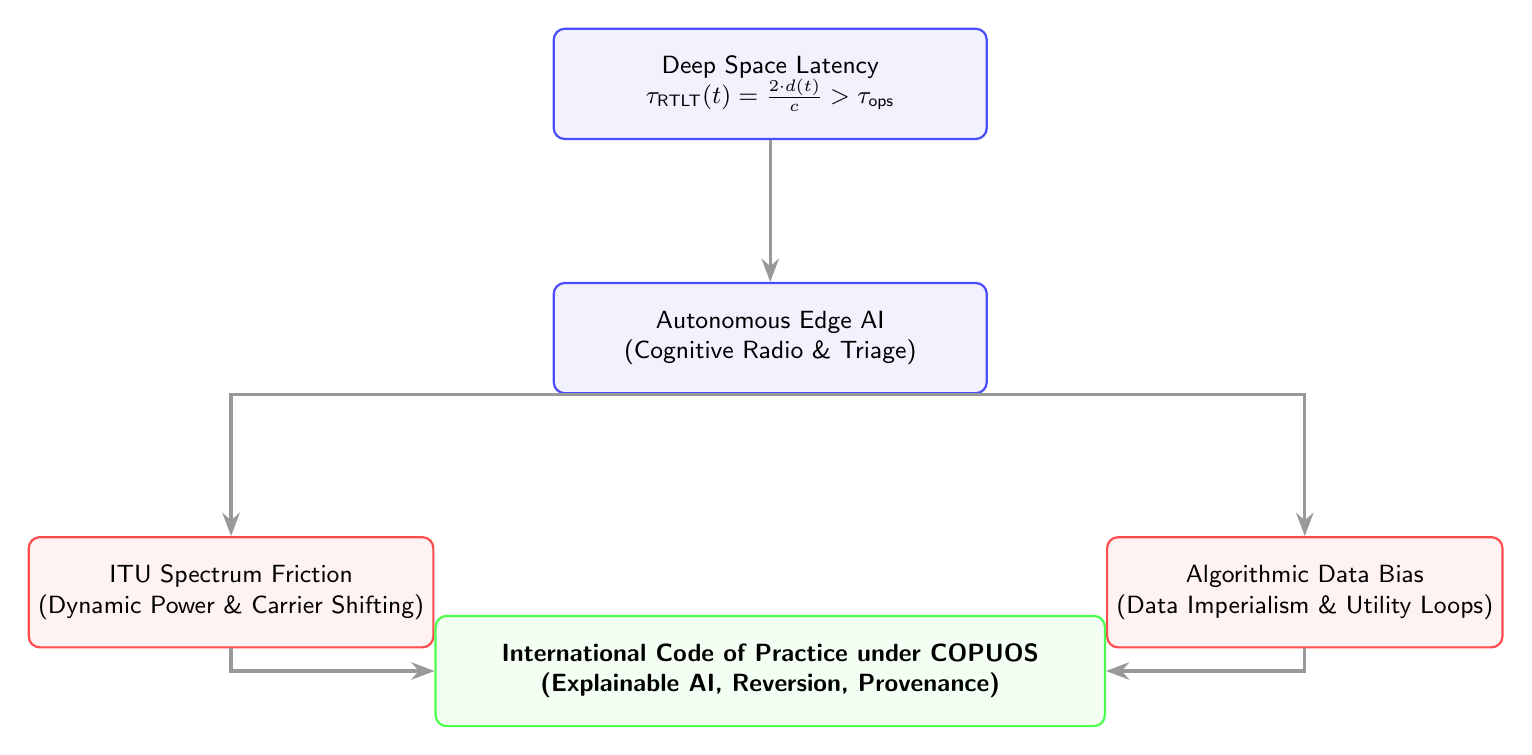
\begin{tikzpicture}[
    node distance=1.8cm and 1.5cm,
    block/.style={
        rectangle, 
        draw=blue!70, 
        fill=blue!5, 
        thick, 
        rounded corners, 
        minimum width=5.5cm, 
        minimum height=1.4cm, 
        align=center,
        font=\sffamily\small
    },
    threat/.style={
        rectangle, 
        draw=red!70, 
        fill=red!5, 
        thick, 
        rounded corners, 
        minimum width=5.0cm, 
        minimum height=1.4cm, 
        align=center,
        font=\sffamily\small
    },
    solution/.style={
        rectangle, 
        draw=green!70, 
        fill=green!5, 
        thick, 
        rounded corners, 
        minimum width=8.5cm, 
        minimum height=1.4cm, 
        align=center,
        font=\sffamily\bfseries\small
    },
    arrow/.style={
        thick, 
        -Stealth, 
        draw=gray!80,
        line width=1.2pt
    }
]
    % Nodes
    \node [block] (latency) {Deep Space Latency\\ $\tau_{\text{RTLT}}(t) = \frac{2 \cdot d(t)}{c} > \tau_{\text{ops}}$};
    \node [block, below=of latency] (ai) {Autonomous Edge AI\\ (Cognitive Radio \& Triage)};
    
    \node [threat, below left=of ai] (itu) {ITU Spectrum Friction\\ (Dynamic Power \& Carrier Shifting)};
    \node [threat, below right=of ai] (triage) {Algorithmic Data Bias\\ (Data Imperialism \& Utility Loops)};
    
    \node [solution, below=2.8cm of ai] (code) {International Code of Practice under COPUOS\\ (Explainable AI, Reversion, Provenance)};

    % Arrows
    \draw [arrow] (latency) -- (ai);
    \draw [arrow] (ai.south) -| (itu.north);
    \draw [arrow] (ai.south) -| (triage.north);
    \draw [arrow] (itu.south) |- (code.west);
    \draw [arrow] (triage.south) |- (code.east);
\end{tikzpicture}
\end{center}

\end{document}
